\section{Análise nodal e análise de malhas}

\frame{
	\frametitle{Métodos de análise}
	\begin{block}{Introdução}
		Tendo compreendido as leis fundamentais da teoria dos circuitos (\textbf{Lei de Ohm} e \textbf{Leis de Kirchhoff}), agora estamos preparados para aplicar essas leis ao desenvolver duas técnicas poderosas para a solução de circuitos: \\
		\begin{enumerate}
			\item \textbf{Análise nodal}: baseia-se em uma aplicação sistemática da \textbf{LKC}.
			\item \textbf{Análise de malhas}: baseia-se em uma aplicação sistemática da \textbf{LKT}.
		\end{enumerate}
	\end{block}
}

\frame{
	\frametitle{Métodos de análise}
	\begin{block}{Sistemas lineares}
		Com as duas técnicas a serem desenvolvidas, teremos condições de analisar qualquer circuito linear pela obtenção de um \textbf{conjunto de equações simultâneas} que são, então, resolvidas para obter os valores necessários de \textbf{corrente} ou \textbf{tensão}.
	\end{block}
}

\frame{
	\frametitle{Análise nodal}
	\begin{block}{Introdução}
		A análise nodal fornece um procedimento genérico para a análise de circuitos usando \textbf{tensões nodais como variáveis de circuitos}. Optar por tensões nodais em vez de tensões de elementos como essas variáveis é conveniente e reduz o número de equações que se deve resolver simultaneamente.
	\end{block}
}

\frame{
	\frametitle{Análise nodal}
	\begin{block}{Etapas}
		\textbf{Na análise nodal estamos interessados em encontrar as tensões nos nós}. Dado um circuito com $n$ nós, sem fontes de tensão, faça: \\
		\begin{enumerate}
			\item Selecione um nó como \textbf{referência}. Atribua tensões $V_1$, $V_2$, ..., $V_{n-1}$ aos $n-1$ nós restantes. As tensões são medidas em relação ao nó de referência.
			      \saveenumerate
		\end{enumerate}
	\end{block}
}

\frame{
	\frametitle{Análise nodal}
	\begin{block}{Etapas}
		\textbf{Na análise nodal estamos interessados em encontrar as tensões nos nós}. Dado um circuito com $n$ nós, sem fontes de tensão, faça: \\
		\begin{enumerate}
			\restoreenumerate
			\item Aplique a \textbf{LKC} a cada um dos $n-1$ nós que não são de referência. Use a \textbf{Lei de Ohm} para expressar as correntes nos ramos em termos de tensões nodais.
			      \saveenumerate
		\end{enumerate}
	\end{block}
}

\frame{
	\frametitle{Análise nodal}
	\begin{block}{Etapas}
		\textbf{Na análise nodal estamos interessados em encontrar as tensões nos nós}. Dado um circuito com $n$ nós, sem fontes de tensão, faça:
		\begin{enumerate}
			\restoreenumerate
			\item \textbf{Resolva as equações simultâneas} resultantes para obter as tensões nodais desconhecidas.
		\end{enumerate}
	\end{block}
}

\frame{
	\frametitle{Análise nodal - Explicação das etapas}
	\begin{block}{Etapa $\#01$}
		O nó de referência é comumente chamado \textbf{terra} (GND), uma vez que se supõe que ele tenha um \textbf{potencial nulo}.
		\begin{itemize}
			\item Assim que escolhemos um nó de referência, atribuímos tensões aos nós que não são de referência.
		\end{itemize}
	\end{block}
	\centerline{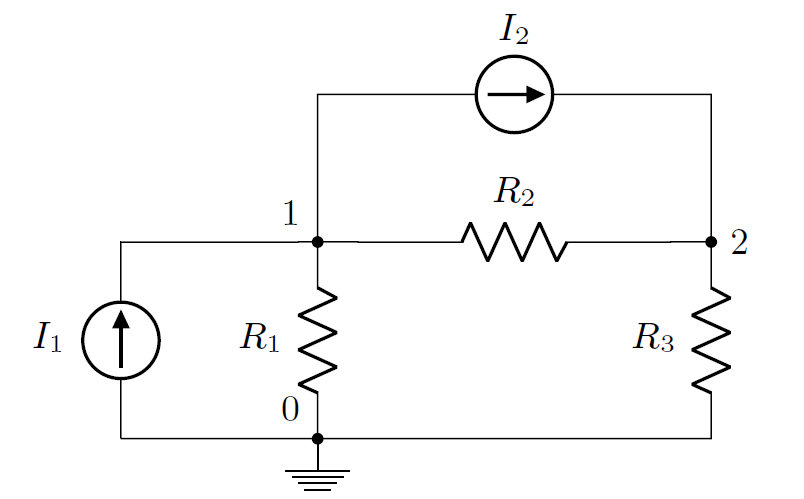
\includegraphics[width=0.6\linewidth]{Figuras/Ch03/fig1.PNG}}
}

\frame{
	\frametitle{Análise nodal - Explicação das etapas}
	\begin{block}{Etapa $\#02$}
		Como segunda etapa, aplicamos a \textbf{LKC} a cada um dos nós que não são de referência do circuito.
		\begin{itemize}
			\itemequation{LKC no \textbf{nó 1}: }{I_1 = I_2 + i_1 + i_2}\label{eqn:2.1}
			\itemequation{LKC no \textbf{nó 2}: }{I_2 + i_2 = i_3}\label{eqn:2.2}
		\end{itemize}
	\end{block}
	\centerline{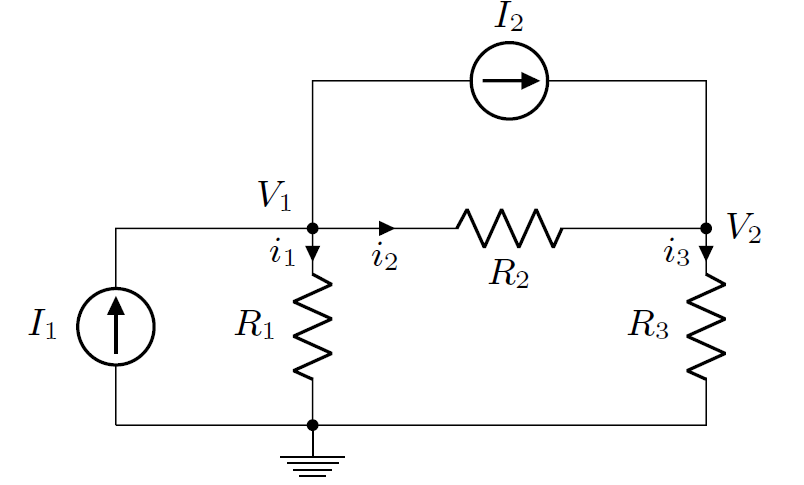
\includegraphics[width=0.6\linewidth]{Figuras/Ch03/fig2.PNG}}
}

\frame{
	\frametitle{Análise nodal - Explicação das etapas}
	\begin{block}{Etapa $\#02$}
		Agora, aplicamos a \textbf{Lei de Ohm} para expressar as correntes desconhecidas $i_1$, $i_2$ e $i_3$ em termos de tensões nodais.
		\begin{itemize}
			\item \textbf{Em um resistor, a corrente flui de um potencial mais elevado para um potencial mais baixo}, isto é, $i = \dfrac{V_{\text{maior}} - V_{\text{menor}}}{R}$
		\end{itemize}

		\vspace{0.2cm}

		\begin{equation}
			i_1 = \dfrac{V_1 - 0}{R_1}\label{eqn:2.3}
		\end{equation}

		\begin{equation}
			i_2 = \dfrac{V_1 - V_2}{R_2}\label{eqn:2.4}
		\end{equation}

		\begin{equation}
			i_3 = \dfrac{V_2 - 0}{R_3}\label{eqn:2.5}
		\end{equation}
	\end{block}
}

\frame{
	\frametitle{Análise nodal - Explicação das etapas}
	\begin{block}{Etapa $\#02$}
		Substituindo as equações \ref{eqn:2.3} a \ref{eqn:2.5} nas equações \ref{eqn:2.1} e \ref{eqn:2.2}, resulta em:
		\vspace{0.2cm}

		\begin{equation}
			I_1 = I_2 + \dfrac{V_1}{R_1} + \dfrac{V_1 - V_2}{R_2}\label{eqn:2.6}
		\end{equation}

		\begin{equation}
			I_2 + \dfrac{V_1 - V_2}{R_2} = \dfrac{V_2}{R_3}\label{eqn:2.7}
		\end{equation}
	\end{block}
}

\frame{
	\frametitle{Análise nodal - Explicação das etapas}
	\begin{block}{Etapa $\#03$}
		A terceira etapa na análise nodal é \textbf{encontrar as tensões nodais}. Se aplicarmos a lei dos nós aos $n-1$ nós que não são de referência, obtemos $n-1$ \textbf{equações simultâneas}, como as equações (6) e (7). Podemos, portanto, obter as tensões nodais $V_1$ e $V_2$ usando qualquer método padrão como o de substituição, eliminação, regra de Cramer ou inversão de matrizes.
	\end{block}
}

\frame{
	\frametitle{Análise nodal - Exemplo \#01}
	\centerline{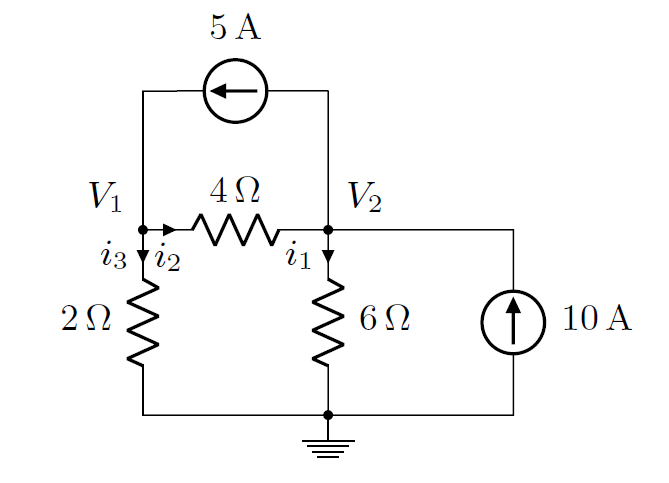
\includegraphics[width=0.55\linewidth]{Figuras/Ch03/fig3.PNG}}
	\begin{block}{Resolução}
		Aplicando \textbf{LKC} e \textbf{Lei de Ohm} no \textbf{Nó 1}: \\
		$$5 = i_2 + i_3 \implies 5 = \dfrac{V_1 - V_2}{4} + \dfrac{V_1 - 0}{2}$$
		$$20 = V_1 - V_2 + 2\cdot V_1 \implies 3 \cdot V_1 - V_2 = 20$$
	\end{block}
}

\frame{
	\frametitle{Análise nodal - Exemplo \#01}
	\centerline{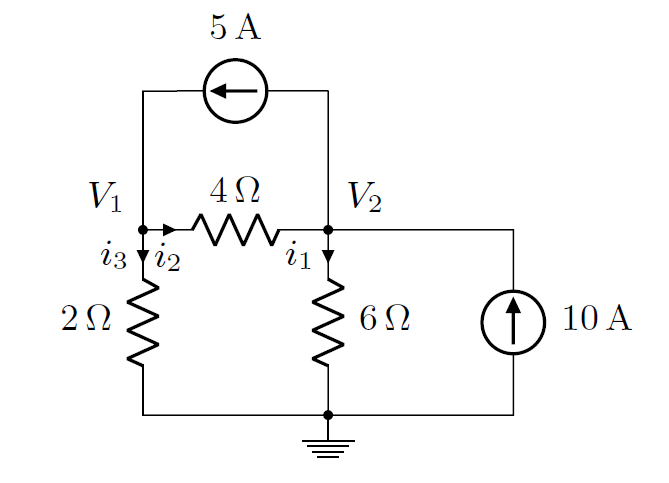
\includegraphics[width=0.55\linewidth]{Figuras/Ch03/fig3.PNG}}
	\begin{block}{Resolução}
		Aplicando \textbf{LKC} e \textbf{Lei de Ohm} no \textbf{Nó 2}: \\
		$$10 + i_2 = 5 + i_1 \implies 10 + \dfrac{V_1 - V_2}{4} = 5 + \dfrac{V_2 - 0}{6}$$
		$$120 + 3 \cdot V_1 - 3 \cdot V_2 = 60 + 2\cdot V_2 \implies -3 \cdot V_1 + 5 \cdot V_2 = 60$$
	\end{block}
}

\frame{
	\frametitle{Análise nodal - Exemplo \#01}
	\begin{block}{Resolução}
		Utilizando a técnica da eliminação, adicionamos as duas equações anteriores:

		$$
			\left\{\begin{aligned}
				3 \cdot V_1  & - V_2         & = 20 \\
				-3 \cdot V_1 & + 5 \cdot V_2 & = 60
			\end{aligned}\right.
		$$

		\vspace{0.2cm}

		Daí, $4 \cdot V_2 = 80 \implies \boxed{V_2 = \SI{20}{\volt}}$ \\
		\vspace{0.2cm}
		Substituindo $V_2 = 20$ V, temos que  $3 \cdot V_1 - 20 = 20 \implies \boxed{V_1 \approx \SI{13.33}{\volt}}$
	\end{block}
}

\frame{
	\frametitle{Análise de malhas}
	\begin{block}{Introdução}
		A análise de malhas fornece outra maneira para a análise de circuitos usando as \textbf{correntes de malha como variáveis do circuito}, em vez de utilizar as correntes de elementos como variáveis. Isto reduz o número de equações que devem ser resolvidas.
		\begin{itemize}
			\item A \textbf{análise nodal} aplica a \textbf{LKC} para encontrar tensões nodais, enquanto a \textbf{análise de malhas} aplica a \textbf{LKT} para determinar correntes desconhecidas.
		\end{itemize}
	\end{block}
}

\frame{
	\frametitle{Análise de malhas}
	\begin{block}{Etapas}
		\textbf{Na análise de malhas estamos interessados em encontrar as correntes de malha}. Dado um circuito com $n$ malhas, faça: \\
		\begin{enumerate}
			\item Atribua \textbf{correntes de malha} $i_1$, $i_2$, ..., $i_n$ a $n$ malhas.
			      \saveenumerate
		\end{enumerate}
	\end{block}
}

\frame{
	\frametitle{Análise de malhas}
	\begin{block}{Etapas}
		\textbf{Na análise de malhas, estamos interessados em encontrar as correntes de malha}. Dado um circuito com $n$ malhas, faça: \\
		\begin{enumerate}
			\restoreenumerate
			\item Aplique a \textbf{LKT} a cada uma das $n$ malhas. Use a \textbf{Lei de Ohm} para expressar as tensões em termos de correntes de malha.
			      \saveenumerate
		\end{enumerate}
	\end{block}
}

\frame{
	\frametitle{Análise de malhas}
	\begin{block}{Etapas}
		\textbf{Na análise de malhas estamos interessados em encontrar as correntes de malha}. Dado um circuito com $n$ malhas, faça: \\
		\begin{enumerate}
			\restoreenumerate
			\item \textbf{Resolva as equações simultâneas} resultantes para obter as correntes de malha desconhecidas.
		\end{enumerate}
	\end{block}
}

\frame{
	\frametitle{Análise de malhas - Explicação das etapas}
	\begin{block}{Etapa $\#01$}
		O primeiro passo requer que as correntes de malha $i_1$ e $i_2$ sejam atribuídas às malhas 1 e 2.
		\begin{itemize}
			\item Embora uma corrente de malha possa ser atribuída a cada malha em seu sentido arbitrário, a convenção diz para supor que cada corrente de malha flua no \textbf{sentido horário}.
		\end{itemize}
	\end{block}
	\centerline{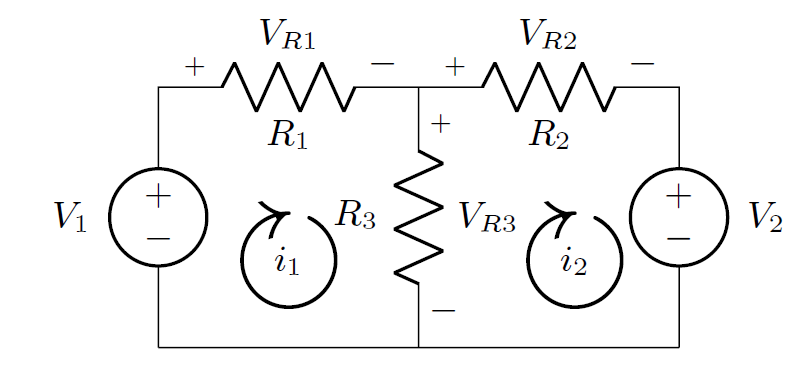
\includegraphics[width=0.6\linewidth]{Figuras/Ch03/fig4.PNG}}
}

\frame{
	\frametitle{Análise de malhas - Explicação das etapas}
	\begin{block}{Etapa $\#02$}
		Como segundo passo, aplicamos a \textbf{LKT} em cada malha.
		\begin{itemize}
			\item LKT na \textbf{malha 1}: $V_1 - R_1 \cdot i_1 - R_3 \cdot (i_1 - i_2) = 0$
			\item LKT na \textbf{malha 2}: $-V_2 -R_2 \cdot i_2 - R_3 \cdot (i_2 - i_1) = 0$
		\end{itemize}
	\end{block}
	\centerline{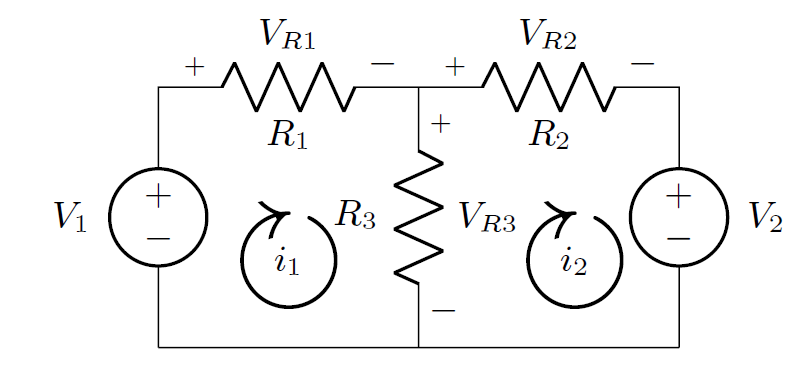
\includegraphics[width=0.6\linewidth]{Figuras/Ch03/fig4.PNG}}
}

\frame{
	\frametitle{Análise de malhas - Explicação das etapas}
	\begin{block}{Etapa $\#03$}
		A terceira etapa é determinar as correntes de malha $i_1$ e $i_2$. Podemos usar qualquer técnica para solucionar as equações simultâneas.
	\end{block}
}

\frame{
	\frametitle{Análise de malhas - Exemplo \#01}
	\centerline{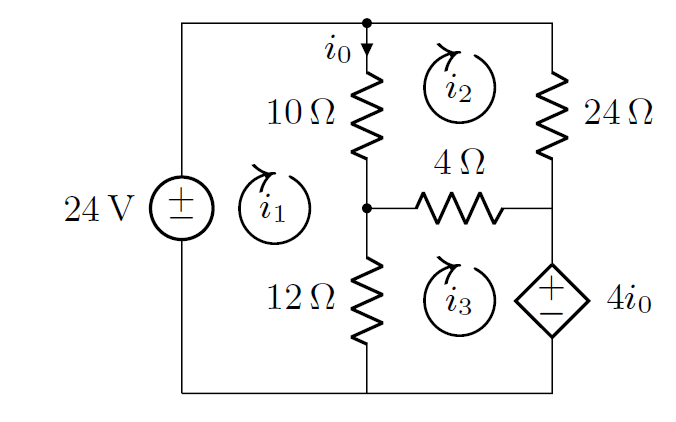
\includegraphics[width=0.55\linewidth]{Figuras/Ch03/fig5.PNG}}
	\begin{block}{Resolução - \textbf{Malha 1}}
		\begin{align*}
		24 - 10 \cdot (i_1 - i_2) - 12 \cdot (i_1 - i_3) &= 0\\
		24 - 10 \cdot i_1 + 10 \cdot i_2 - 12 \cdot i_1 + 12 \cdot i_3 &= 0\\
		- 22 \cdot i_1 + 10 \cdot i_2 + 12 \cdot i_3 &= -24\\
		11 \cdot i_1 - 5 \cdot i_2 - 6 \cdot i_3 &= 12
		\end{align*}
		
	\end{block}
}

\frame{
	\frametitle{Análise de malhas - Exemplo \#01}
	\centerline{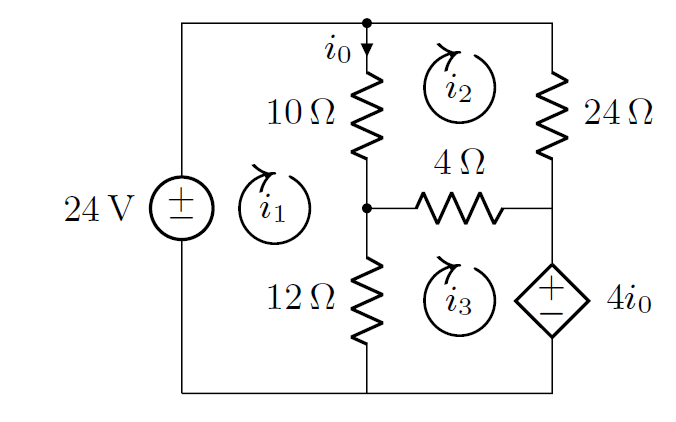
\includegraphics[width=0.55\linewidth]{Figuras/Ch03/fig5.PNG}}
	\begin{block}{Resolução - \textbf{Malha 2}}
		\begin{align*}
			- 10 \cdot (i_2 - i_1) - 24 \cdot i_2 - 4 \cdot (i_2 - i_3) &= 0\\
			- 10 \cdot i_2 + 10 \cdot i_1 - 24 \cdot i_2 - 4 \cdot i_2 + 4 \cdot i_3 &= 0\\
			10 \cdot i_1 - 38 \cdot i_2 + 4 \cdot i_3 &= 0\\
			5 \cdot i_1 - 19 \cdot i_2 + 2 \cdot i_3 &= 0
		\end{align*}
	\end{block}
}

\frame{
	\frametitle{Análise de malhas - Exemplo \#01}
	\centerline{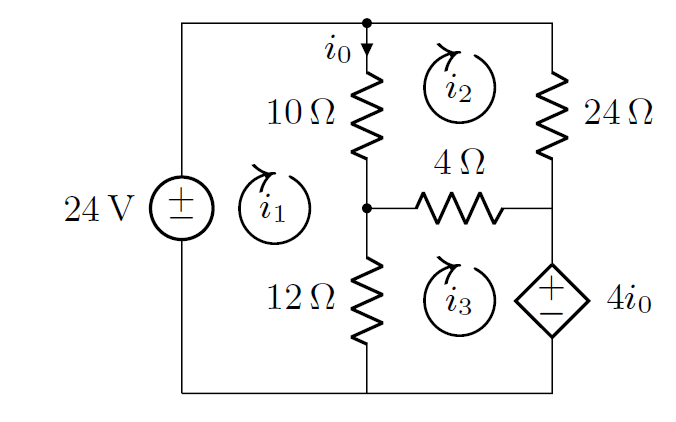
\includegraphics[width=0.55\linewidth]{Figuras/Ch03/fig5.PNG}}
	\begin{block}{Resolução - \textbf{Malha 3}}
		\begin{align*}
			-4 \cdot i_0 - 12 \cdot (i_3 - i_1) - 4 \cdot (i_3 - i_2) &= 0\\
			-4 \cdot (i_1 - i_2) - 12 \cdot (i_3 - i_1) - 4 \cdot (i_3 - i_2) &= 0\\
			-4 \cdot i_1 +4 \cdot i_2 - 12 \cdot i_3 + 12 \cdot i_1 - 4 \cdot i_3 + 4 \cdot i_2 &= 0\\
			i_1 + i_2 - 2 \cdot i_3 &= 0
		\end{align*}
	\end{block}
}

\frame{
	\frametitle{Análise de malhas - Exemplo \#01}
	\begin{block}{Regra de Cramer}
		\begin{equation*}
			\begin{bmatrix}
				11 & -5  & -6 \\
				5  & -19 & 2  \\
				1  & 1   & -2 \\
			\end{bmatrix}
			\begin{bmatrix}
				i_1 \\
				i_2 \\
				i_3 \\
			\end{bmatrix}
			=
			\begin{bmatrix}
				\textcolor{red}{12} \\
				\textcolor{red}{0}  \\
				\textcolor{red}{0}  \\
			\end{bmatrix}
		\end{equation*}

		\vspace{0.5cm}

		\begin{equation*}
			\Delta = \begin{vmatrix}
				11 & -5  & -6 \\
				5  & -19 & 2  \\
				1  & 1   & -2 \\
			\end{vmatrix}
			= 192
		\end{equation*}
	\end{block}
}

\frame{
	\frametitle{Análise de malhas - Exemplo \#01}
	\begin{block}{Regra de Cramer}

		\begin{align*}
			\Delta_{\textcolor{red}{1}} &= \begin{vmatrix}
				\textcolor{red}{12} & -5  & -6 \\
				\textcolor{red}{0}  & -19 & 2  \\
				\textcolor{red}{0}  & 1   & -2
			\end{vmatrix}
			= 432 \\
			\Delta_{\textcolor{red}{2}} &= \begin{vmatrix}
			11 & \textcolor{red}{12} & -6 \\
			5  & \textcolor{red}{0}  & 2  \\
			1  & \textcolor{red}{0}  & -2
			\end{vmatrix}
			= 144 \\
			\Delta_{\textcolor{red}{3}} &= \begin{vmatrix}
			11 & -5  & \textcolor{red}{12} \\
			5  & -19 & \textcolor{red}{0}  \\
			1  & 1   & \textcolor{red}{0}
			\end{vmatrix}
			= 288
		\end{align*}

		\begin{align*}
			i_1 &= \dfrac{\Delta_1}{\Delta} = \SI{2.25}{\ampere}  & i_2 &= \dfrac{\Delta_2}{\Delta} = \SI{0.75}{\ampere} & i_3 &= \dfrac{\Delta_3}{\Delta} = \SI{1.5}{\ampere}
		\end{align*}
		
		Com isso, $\boxed{i_0 = i_1 - i_2 = \SI{1.5}{\ampere}}$

	\end{block}
}

\section*{Exercícios}
\frame{
	\frametitle{Exercícios}
	\begin{block}{}
		01. Determine as tensões $V_1$ e $V_2$ utilizando a análise nodal. \\
		\vspace{0.3cm}
		\centerline{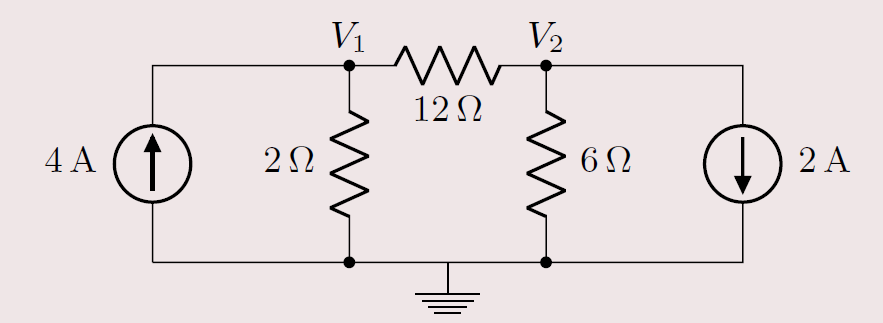
\includegraphics[width=0.8\linewidth]{Figuras/Ch03/fig6.PNG}}
	\end{block}
}

\section*{Exercícios}
\frame{
	\frametitle{Exercícios}
	\begin{block}{}
		02. Para o circuito abaixo, determine as correntes de ramo $i_1$, $i_2$ e $i_3$ usando a análise de malhas. \\
		\vspace{0.3cm}
		\centerline{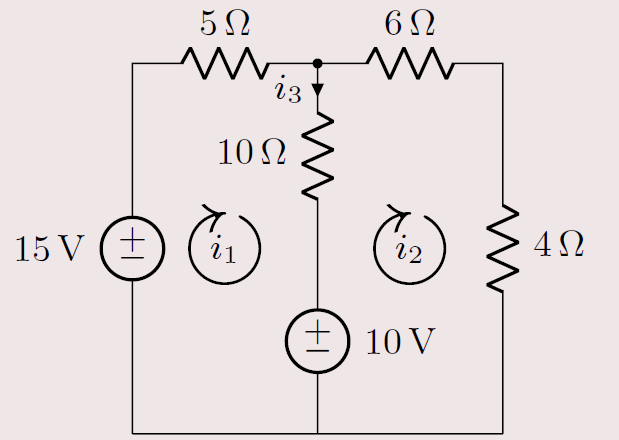
\includegraphics[width=0.6\linewidth]{Figuras/Ch03/fig7.PNG}}
	\end{block}
}

\section*{Referências}

\frame{
	\frametitle{Referências e Exercícios Complementares}
	\begin{itemize}
		\item ALEXANDRE, Charles K.; SADIKU, Matthew N. O. Fundamentos de Circuitos Elétricos. 5. ed. Porto Alegre: AMGH, 2013.
	\end{itemize}
	%\centering{\alert{Página 36 - \textbf{1.6.1 até 1.6.5, 1.6.17 até 1.6.19}}} \\
	\centering{\alert{Lista de exercícios 03}}
}